\chapter{Design}
\label{chap:design}
In Chapter \ref{chap:threat_model}, we discussed the threat modelling and risk analysis of an OpenID Connect application implemented using PKCE on a cloud environment. The threat modelling provided an in-depth understanding of potential attack vectors and risks that could compromise the cloud-based application using the OpenID Connect Protocol. Building upon the insights gathered from the threat modelling exercise (See \ref{subsec:stride}), this chapter will focus on designing a prototype to address some identified threats. In particular, the very high and high threats will be mitigated. See Table \ref{table:risk_assessment}. 

This chapter will outline the implementation decisions and design choices undertaken to address identified risks. The objective is to establish a secure, scalable, and efficient cloud-based authentication system utilising Proof Key for Code Exchange (PKCE) on Amazon Web Services (AWS).

\section{Cloud Provider}
\label{sec:cloud_provider}
Designing and deploying a cloud-based application requires us to choose one of the many providers that offer such services as Microsoft Azure, Google Cloud Platform (GCP), and Amazon Web Services (AWS). Each of these popular platforms offers unique advantages and different service offerings. 

However, for this project, AWS is the preferred platform as it is the leader in the cloud services industry, with a vast global infrastructure that ensures reliability and scalability. \cite{aws_leader} states that it holds the most shares as a favoured vendor, with 31 per cent in the first quarter of 2024. Not only is AWS a widely adopted cloud platform, but it is also compliant with ISO 27001 and GDPR \citep{aws_iso}. In addition to the advantages of compliance, AWS offers extensive tools for prototyping and testing, namely Localstack.

\subsection{LocalStack for AWS Simulation}
LocalStack is a tool that allows developers to simulate AWS services locally, making it an excellent choice for rapid development and testing. With LocalStack, developers can build applications locally using AWS-like services such as Lambda, API Gateway, and more without needing to deploy code to the cloud \citep{localstack}. By mimicking the AWS environment, LocalStack allows developers to work on cloud-native applications locally, reducing development costs and the need to register for an AWS account, which is cost-intensive. Such a simulation tool does not yet exist for Azure and GCP, creating a solid argument for using AWS.


\subsection{Limitations}
\begin{itemize}
    \item \textbf{Partial Service Emulation}: 
    LocalStack does not fully emulate all AWS services or features. Specific service behaviours might not be available or behave differently than in the AWS environment.
    
    \item \textbf{Performance Differences}: 
    Since LocalStack runs locally, its performance might not accurately reflect the AWS cloud's.
    
    
    \item \textbf{Version Mismatches}: 
    LocalStack may not continuously be updated in sync with AWS's latest services and API changes, potentially causing discrepancies between local development and production deployments.
    
    \item \textbf{Complex Setup}: 
    As application architectures grow more complex, configuring and maintaining a Local Stack with multiple services can become challenging and time-consuming. In addition, to run a local stack, one must understand and learn how to spin up an environment with required services. For example, one must also understand the principles of running and managing docker containers.
    
    \item \textbf{Limited Real-World Testing}: 
    While LocalStack is excellent for early development and testing, certain edge cases or AWS-specific behaviours may only be encountered in the natural cloud environment, necessitating additional testing after deployment.
    
\end{itemize}

\section{Architecture}
After deciding to use AWS as the cloud provider in Section \ref{sec:cloud_provider}, the application's design is centred around AWS services such as API Gateway, Lambda Servers, and DynamoDB for the database. In this section, we will delve into the chosen services in detail. The deployment of the PKCE (Proof Key for Code Exchange) application for two tenants necessitates a database to store user data. For this project, we have evaluated two different approaches for a multi-tenant setup: one involving a single database with data isolation and another involving multiple databases per tenant (Refer to Figures \ref{fig:deployment_diagram_single} and \ref{fig:deployment_diagram_dual}).



In \cite{niemela2023implementing}, the advantages and disadvantages of single and multiple databases per tenant are discussed. It argues that the multi-tenant application with multiple databases balances performance and security. This approach allows the databases to scale according to the needs of each tenant. It provides the capability to implement granular security measures such as encrypting specific data, maintaining access controls, and generating clear access logs. These features reinforce the data model's Confidentiality, Integrity, and Availability (CIA) principle. However, this approach also has drawbacks compared to its single database counterpart. Managing multiple databases introduces overhead and increases the likelihood of misconfiguration, as each database operates independently. Despite the additional configuration and maintenance complexity, the approach with multiple databases is a viable solution for the application. The security benefits of using multiple databases are as follows:

\begin{itemize}
    \item \textbf{Isolation of Sensitive Data}: Unlike a single database for a multi-tenant application, the data are isolated from each other entirely. Should a security vulnerability be discovered, the damage will be limited to one data set rather than exposing all sensitive information. 
    
    \item \textbf{Improved performance}: Separation of tenant data allows a more efficient way of accessing the data. Using one table in the database does not affect the other. Furthermore, the database can be configured according to each tenant's needs to scale it up and down, increasing performance. This, in terms of simplifying the queries to retrieve data, also reduces possible SQL attacks due to more straightforward queries.
    
    \item \textbf{Custom Encryption Keys}: Using two tables, separate encryption keys for each table, enhancing the data security and ensuring that each data set has independent encryption controls that can be configured. Should one encryption key be compromised, the other remains secure. 
 
\end{itemize}

\begin{figure}[h!]
\label{fig:deployment_diagram_single}
\centering
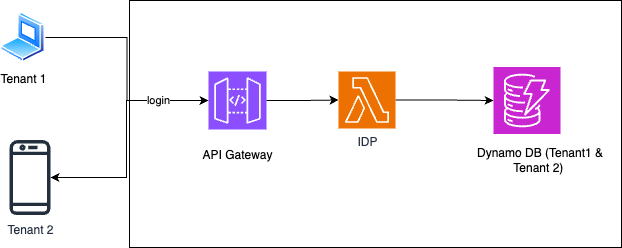
\includegraphics[width=\textwidth, height=200px]{pics/deployment_diagram_single.png}
\caption{Deployment diagram with Single Database}
\end{figure}

\begin{figure}[h!]
\centering
\label{fig:deployment_diagram_dual}
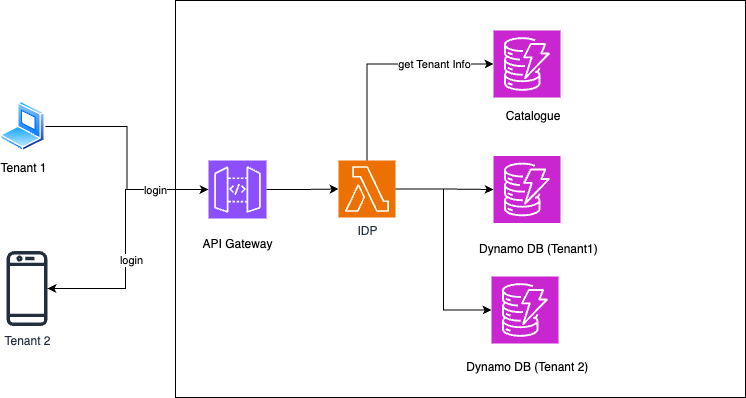
\includegraphics[width=\textwidth, height=200px]{pics/deployment_diagram.dual.png}
\caption{Deployment diagram with Multi Database}
\end{figure}

\subsection{Overview of the Deployment Architecture}
This section discusses the AWS services used to implement the PKCE flow for two tenants with multiple databases (See Figure \ref{fig:deployment_diagram_dual}). The deployment architecture consists of the following main components:

\begin{itemize}
    \item \textbf{API Gateway}: This is the public interface for the application that provides endpoints for the clients to perform login and authorisation. This service is responsible for routing the requests to the appropriate Lambda based on the path. The API gateway can also be configured to restrict access using the API key and limit the request using throttling, preventing unwanted access and reducing Denial of Service attacks.
    
    \item \textbf{Lambda Functions}: Lambda functions are serverless functions that contain the logic that handles the PKCE OpenID Connect. It is responsible for storing and retrieving the PKCE code verifiers, processing the callback, authenticating and authorising users, and generating access and refresh tokens. In contrast to regular servers, Lambdas are more lightweight, spun up only when needed, and terminated after their runtime. In addition, AWS Lambdas uses a specialised virtual machine manager (VMM) called Firecracker, which helps with container isolation, as AWS uses shared hardware protecting from microarchitectural attacks \citep{lambda_vm_firecracker}. Advantages such as resource optimization and the lack of container orchestration and setup for the prototype make it a proper candidate.
    
    \item \textbf{DynamoDB Databases}: DynamoDB is a AWS proprietary NOSQL database. This database is used as it is easy to use and can be easily integrated with the other services that would speed up the implementation of the prototype. These databases will store user-specific data, such as user information and credentials, and code verifiers associated with each user session. The database is configured per tenant so that each tenant will have a database. By storing PKCE code verifiers and tenant data in separate tables, we can isolate sensitive information based on its purpose. If one table’s access were compromised, the other table’s data would remain secure. This is particularly useful when dealing with data regulated under compliance frameworks like GDPR or HIPAA, as it helps limit data exposure. DynamoDB, also like AWS lambda, abstracts away all server management and provisioning tasks \citep{dynamodb}. Therefore, using Dynamodb allows more flexibility and complex SQL queries are not required for data structure as they can be stored in a flexible schema design and fit the project.

\end{itemize}


Deploying an application using AWS API Gateway, AWS Lambda, and multiple DynamoDB tables offers a highly secure and scalable architecture that aligns with modern best practices for serverless computing and data protection. A key advantage of using two distinct DynamoDB tables is the ability to isolate different types of data based on their sensitivity or usage patterns. For instance, sensitive data such as personally identifiable information (PII) can be stored in one table, while less critical operational data resides in another. This separation enhances security by reducing the risk of unauthorized access or exposure; if a breach occurs, the impact is contained to only one table, making it easier to manage and mitigate damage. Additionally, this setup allows for applying granular IAM (Identity and Access Management) policies, enabling fine-tuned control over who or what can access each table. This granular approach enforces the principle of least privilege, ensuring that users and services only have the permissions they need, ultimately minimizing the risk of accidental or malicious access to sensitive data. The ability to tailor permissions at the table level makes it far easier to implement strict security measures, which is especially important for organisations handling sensitive information or subject to stringent regulatory requirements.



